\documentclass[PianoDiProgetto.tex]{subfiles}
%TODO sistemare tabelle e immagini
\begin{document}	
% per tabelle, alterna i colori delle righe		
\taburowcolors[2] 2{tableLineOne .. tableLineTwo}
\tabulinesep = ^3mm_2mm

\chapter{Suddivisione risorse e preventivo}
\section{Analisi}
\subsection{Prospetto Orario}
Nel periodo di Analisi la distribuzione oraria è la seguente:
\begin{table}[H]
	\begin{center}
		\begin{tabu} to \textwidth {
				>{\centering}m{0.3\linewidth} 
				>{\centering}m{0.05\linewidth}  
				>{\centering}m{0.05\linewidth}  
				>{\centering}m{0.05\linewidth}
				>{\centering}m{0.05\linewidth}
				>{\centering}m{0.05\linewidth}
				>{\centering}m{0.05\linewidth}
				>{\centering\arraybackslash}m{0.15\linewidth}
			}
			\tableHeaderStyle			
			\textbf{Nome} & \textbf{Re} & \textbf{Ad} & \textbf{An} & \textbf{Pj} & \textbf{Pr} & \textbf{Ve} & \textbf{Totale} \\
			\Davide &  & 11 & 4 &  &  & 10 & 25 \\
			\Elena & 10 & 8 & 3 &  &  & 4 & 25 \\
			\Gianluca &  & 2 & 15 &  &  & 8 & 25 \\
			\Mirco &  & 4 & 16 &  &  & 5 & 25 \\
			\Parwinder & 8 & 8 & 3 &  &  & 6 & 25 \\
			\Riccardo &  & 11 & 4 &  &  & 10 & 25 \\
			\Valentina & 5 & 8 & 4 &  &  & 8 & 25 \\
		\end{tabu}
		\caption{Distribuzione oraria del periodo di Analisi}
		\vspace{-1em}
	\end{center}
\end{table}
\newpage	
Il seguente grafico dà una rappresentazione visiva della suddivisione oraria:
\begin{figure}[h]
	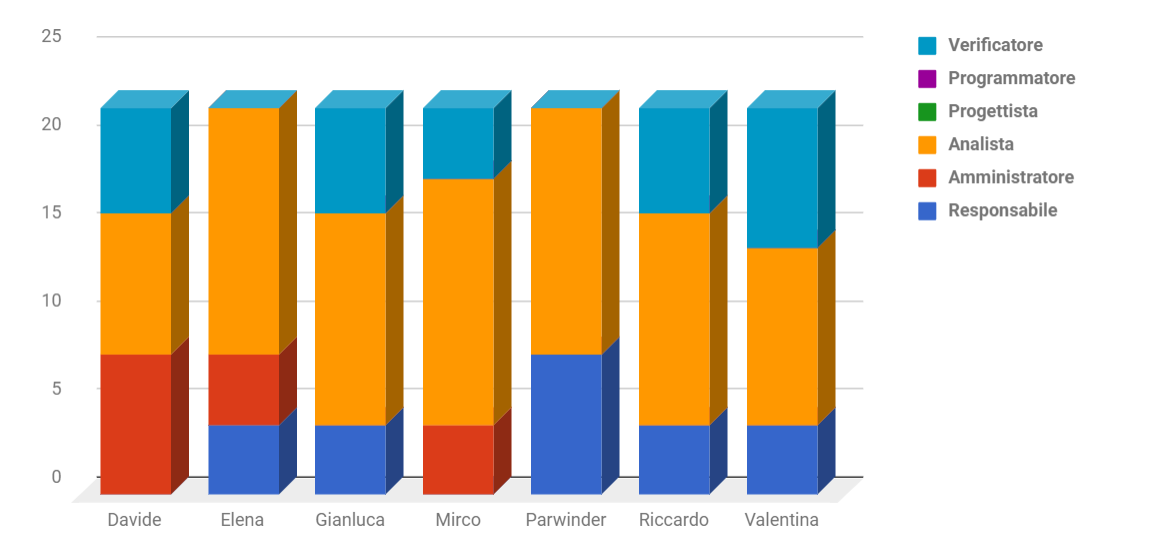
\includegraphics[width=14.5cm]{images/prospettoOrario/analisi.png}
	\label{fig:foo}
	\caption{Grafico suddivisione oraria del periodo di Analisi}
\end{figure} 

\subsection{Prospetto Economico}
Nel periodo di Analisi la distribuzione delle ore tra i differenti ruoli è la seguente:\\
\begin{table}[H]
	\begin{center}
		\capstart
		\begin{tabu} to \textwidth { 
				>{\centering}m{0.4\linewidth} 
				>{\centering}m{.2\linewidth}  
				>{\centering\arraybackslash}m{0.25\linewidth}  }
			\tableHeaderStyle
			\textbf{Ruolo} & \textbf{Ore} & \textbf{Costo in \euro} \\
			\resp & 23 & 690,00 \\
			\amme & 52 & 1.040,00 \\
			\alista & 49 & 1.225,00 \\
			\proga &  &  \\
			\progre &  &  \\
			\vere & 51 & 765,00 \\
			\textbf{Totale} & \textbf{175} & \textbf{3.720,00} \\
		\end{tabu}
		\caption{Prospetto economico del periodo di Analisi}
		\vspace{-1em}
	\end{center}
\end{table}
\newpage
Il seguente grafico dà una rappresentazione visiva della distribuzione dei ruoli:
\begin{figure}[h]
	\centering
	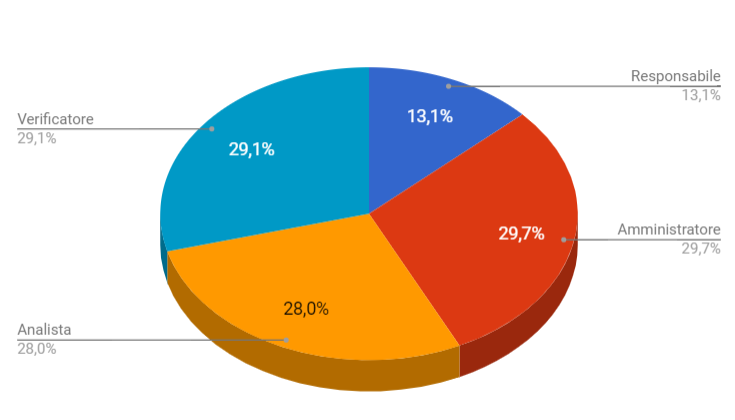
\includegraphics[width=10.5cm]{images/prospettoEconomico/analisi.png}
	\label{fig:foo}
	\caption{Grafico suddivisione dei ruoli del periodo di Analisi}
\end{figure} 
\section{Consolidamento dei requisiti}
\subsection{Prospetto Orario}
Nel periodo di Consolidamento dei requisiti la distribuzione oraria è la seguente:
\begin{table}[H]
	\begin{center}
		\begin{tabu} to \textwidth {
				>{\centering}m{0.3\linewidth} 
				>{\centering}m{0.05\linewidth}  
				>{\centering}m{0.05\linewidth}  
				>{\centering}m{0.05\linewidth}
				>{\centering}m{0.05\linewidth}
				>{\centering}m{0.05\linewidth}
				>{\centering}m{0.05\linewidth}
				>{\centering\arraybackslash}m{0.15\linewidth}
			}
			\tableHeaderStyle			
			\textbf{Nome} & \textbf{Re} & \textbf{Ad} & \textbf{An} & \textbf{Pj} & \textbf{Pr} & \textbf{Ve} & \textbf{Totale} \\
			\Davide 	&  & 3 & 4 &  &  &  & 7 \\
			\Elena 		&  &  & 2 &  &  & 5 & 7 \\
			\Gianluca 	&  &  &  &  &  & 7 & 7 \\
			\Mirco		&  & 4 & 3 &  &  &  & 7 \\
			\Parwinder	&  &  & 7 &  &  & 6 & 7 \\
			\Riccardo 	& 5 & 2 & 4 &  &  &  & 7 \\
			\Valentina	&  &  &  &  &  & 7 & 7 \\
		\end{tabu}
		\caption{Distribuzione oraria del periodo di Consolidamento dei requisiti}
		\vspace{-1em}
	\end{center}
\end{table}
\newpage
Il seguente grafico dà una rappresentazione visiva della suddivisione oraria:
\begin{figure}[h]
	\centering
	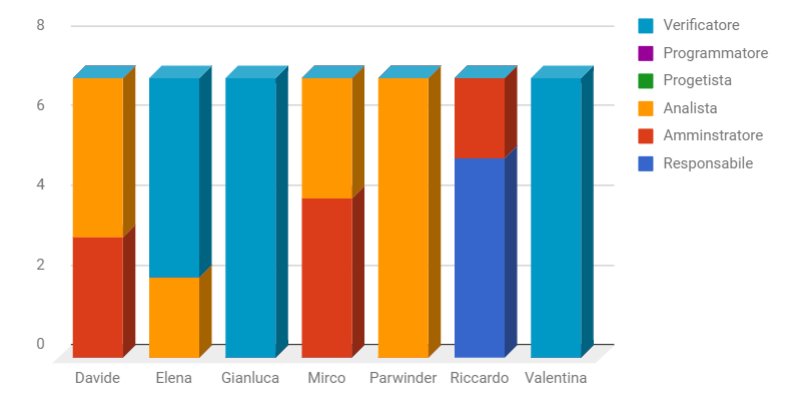
\includegraphics[width=12.5cm]{images/prospettoOrario/consolidamento.png}
	\label{fig:foo}
	\caption{Grafico suddivisione oraria del periodo di Consolidamento dei requisiti}
\end{figure} 
\subsection{Prospetto Economico}
Nel periodo di Analisi la distribuzione delle ore tra i differenti ruoli è la seguente:
\begin{table}[H]
	\begin{center}
		\capstart
		\begin{tabu} to \textwidth { 
				>{\centering}m{0.4\linewidth} 
				>{\centering}m{.2\linewidth}  
				>{\centering\arraybackslash}m{0.25\linewidth}  }
			\tableHeaderStyle
			\textbf{Ruolo} & \textbf{Ore} & \textbf{Costo in \euro} \\
			\resp & 5 & 120,00 \\
			\amme & 9 & 180,00 \\
			\alista & 16 & 400,00 \\
			\proga &  &  \\
			\progre &  &  \\
			\vere & 19 & 285,00 \\
			\textbf{Totale} & \textbf{49} & \textbf{985,00} \\
		\end{tabu}
		\caption{Prospetto economico del periodo di Consolidamento dei requisiti}
		\vspace{-1em}
	\end{center}
\end{table}
\clearpage
Il seguente grafico dà una rappresentazione visiva della distribuzione dei ruoli:
\begin{figure}[h]
	\centering
	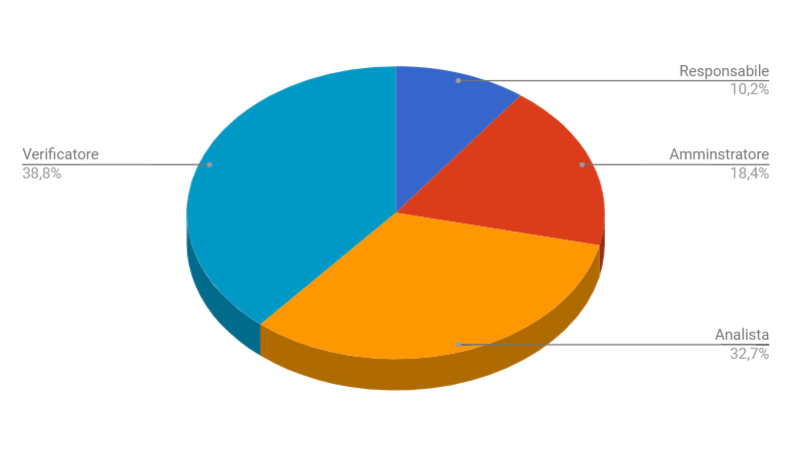
\includegraphics[width=10.5cm]{images/prospettoEconomico/consolidamento.png}
	\label{fig:foo}
	\caption{Grafico suddivisione dei ruoli del periodo di Consolidamento dei requisiti}
\end{figure} 
\clearpage
\section{Progettazione della base tecnologica}
\subsection{Prospetto Orario}
Nel periodo di Progettazione architetturale la distribuzione oraria è la seguente:
\begin{table}[H]
	\begin{center}
		\begin{tabu} to \textwidth {
				>{\centering}m{0.3\linewidth} 
				>{\centering}m{0.05\linewidth}  
				>{\centering}m{0.05\linewidth}  
				>{\centering}m{0.05\linewidth}
				>{\centering}m{0.05\linewidth}
				>{\centering}m{0.05\linewidth}
				>{\centering}m{0.05\linewidth}
				>{\centering\arraybackslash}m{0.15\linewidth}
			}
			\tableHeaderStyle			
			\textbf{Nome} & \textbf{Re} & \textbf{Ad} & \textbf{An} & \textbf{Pj} & \textbf{Pr} & \textbf{Ve} & \textbf{Totale} \\
			\Davide 	& 8 &  & 10 &  & 6 & 6 & 30 \\
			\Elena 		&  &  &  & 14 & 6 & 10 & 30 \\
			\Gianluca 	&  & 5 &  &  & 10 & 15 & 30 \\
			\Mirco		&  &  &  & 12 & 10 & 8 & 30 \\
			\Parwinder	&  &  &  & 6 & 10 & 14 & 30 \\
			\Riccardo 	& 5 &  &  & 9 & 6 & 10 & 30 \\
			\Valentina	&  & 5 & 10 &  & 6 & 9 & 30 \\
		\end{tabu}
		\caption{Distribuzione oraria del periodo di Progettazione della base tecnologica}
		\vspace{-1em}
	\end{center}
\end{table}
Il seguente grafico dà una rappresentazione visiva della suddivisione oraria:
\begin{figure}[h]
	\centering
	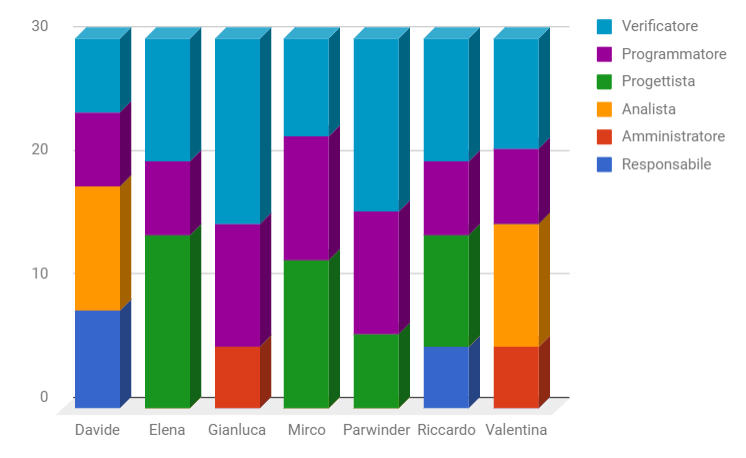
\includegraphics[width=10.5cm]{images/prospettoOrario/progArch.png}
	\label{fig:foo}
	\caption{Grafico suddivisione oraria del periodo di Progettazione architetturale}
\end{figure} 
\newpage
\subsection{Prospetto Economico}
Nel periodo di Progettazione della base tecnologica la distribuzione delle ore tra i differenti ruoli è la seguente:
\begin{table}[H]
	\begin{center}
		\capstart
		\begin{tabu} to \textwidth { 
				>{\centering}m{0.4\linewidth} 
				>{\centering}m{.2\linewidth}  
				>{\centering\arraybackslash}m{0.25\linewidth}  }
			\tableHeaderStyle
			\textbf{Ruolo} & \textbf{Ore} & \textbf{Costo in \euro} \\
			\resp & 13 & 390,00 \\
			\amme & 10 & 200,00 \\
			\alista & 20 & 500,00 \\
			\proga & 41 & 902,00 \\
			\progre & 54 & 810,00 \\
			\vere & 72 & 1.080,00 \\
			\textbf{Totale} & \textbf{210} & \textbf{3.882,00} \\
		\end{tabu}
		\caption{Prospetto economico del periodo di Consolidamento dei requisiti}
		\vspace{-1em}
	\end{center}
\end{table}
Il seguente grafico dà una rappresentazione visiva della distribuzione dei ruoli:
\begin{figure}[h]
	\centering
	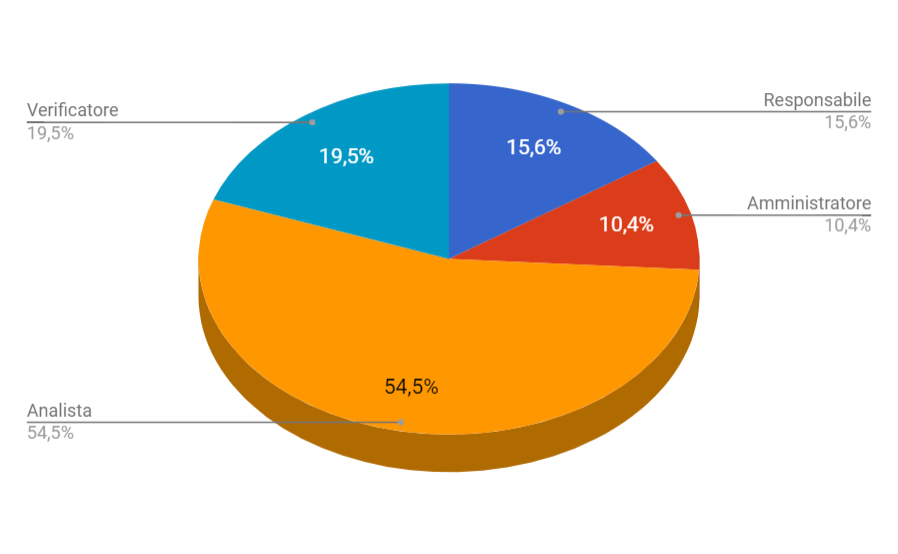
\includegraphics[width=10.5cm]{images/prospettoEconomico/progArch.png}
	\label{fig:foo}
	\caption{Grafico suddivisione dei ruoli del periodo di Progettazione architetturale}
\end{figure} 
\newpage
\section{Progettazione di dettaglio e codifica}
\subsection{Prospetto Orario}
Nel periodo di Progettazione di dettaglio e codifica la distribuzione oraria è la seguente:
\begin{table}[H]
	\begin{center}
		\begin{tabu} to \textwidth {
				>{\centering}m{0.3\linewidth} 
				>{\centering}m{0.05\linewidth}  
				>{\centering}m{0.05\linewidth}  
				>{\centering}m{0.05\linewidth}
				>{\centering}m{0.05\linewidth}
				>{\centering}m{0.05\linewidth}
				>{\centering}m{0.05\linewidth}
				>{\centering\arraybackslash}m{0.15\linewidth}
			}
			\tableHeaderStyle			
			\textbf{Nome} & \textbf{Re} & \textbf{Ad} & \textbf{An} & \textbf{Pj} & \textbf{Pr} & \textbf{Ve} & \textbf{Totale} \\
			\Davide 	&  &  &  & 17 & 20 & 15 & 52 \\
			\Elena 		&  &  & 4 & 18 & 20 & 10 & 52 \\
			\Gianluca 	&  & 8 &  & 16 & 18 & 10 & 52 \\
			\Mirco		& 8 &  &  & 16 & 18 & 10 & 52 \\
			\Parwinder	&  &  &  & 24 & 18 & 10 & 52 \\
			\Riccardo 	&  &  & 4 & 16 & 20 & 12 & 52 \\
			\Valentina	& 5 &  &  & 27 & 20 &  & 52 \\
		\end{tabu}
		\caption{Distribuzione oraria del periodo di Progettazione in dettaglio e codifica}
		\vspace{-1em}
	\end{center}
\end{table}
Il seguente grafico dà una rappresentazione visiva della suddivisione oraria:
\begin{figure}[h]
	\centering
	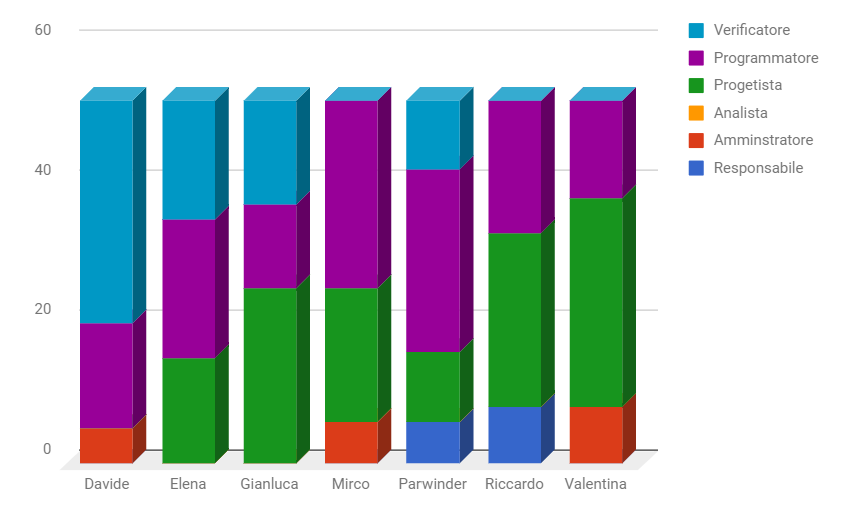
\includegraphics[width=10.5cm]{images/prospettoOrario/progCod.png}
	\label{fig:foo}
	\caption{Grafico suddivisione oraria del periodo di Progettazione di dettaglio e codifica}
\end{figure} 
\newpage
\subsection{Prospetto Economico}
Nel periodo di Progettazione di dettaglio e codifica la distribuzione delle ore tra i differenti ruoli è la seguente:
\begin{table}[H]
	\begin{center}
		\capstart
		\begin{tabu} to \textwidth { 
				>{\centering}m{0.4\linewidth} 
				>{\centering}m{.2\linewidth}  
				>{\centering\arraybackslash}m{0.25\linewidth}  }
			\tableHeaderStyle
			\textbf{Ruolo} & \textbf{Ore} & \textbf{Costo in \euro} \\
			\resp & 13 & 390,00 \\
			\amme & 8 & 160,00 \\
			\alista & 8 & 200,00 \\
			\proga & 134 & 2.948,00 \\
			\progre & 134 & 2.010,00 \\
			\vere & 67 & 1.005,00 \\
			\textbf{Totale} & \textbf{364} & \textbf{6.713,00} \\
		\end{tabu}
		\caption{Prospetto economico del periodo di Progettazione di dettaglio e codifica}
		\vspace{-1em}
	\end{center}
\end{table}
Il seguente grafico dà una rappresentazione visiva della distribuzione dei ruoli:
\begin{figure}[h]
	\centering
	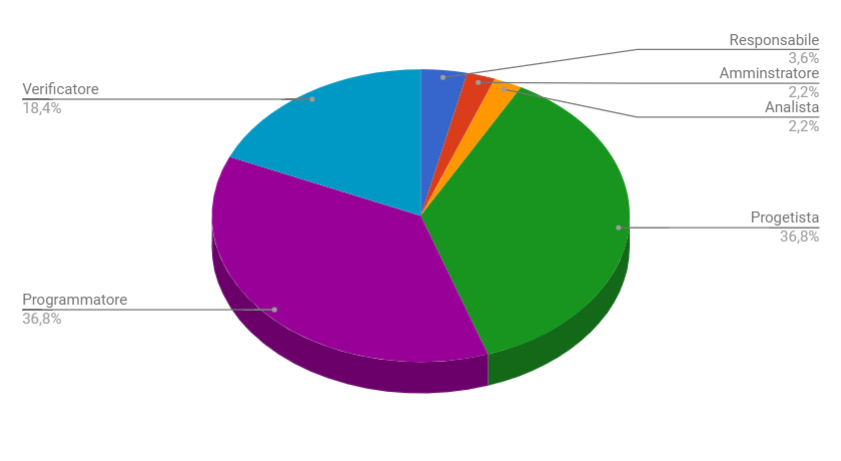
\includegraphics[width=12cm]{images/prospettoEconomico/progCod.png}
	\label{fig:foo}
	\caption{Grafico suddivisione dei ruoli del periodo di Progettazione di dettaglio e codifica}
\end{figure} 
\clearpage

\section{Validazione e collaudo}
\subsection{Prospetto Orario}
Nel periodo di Validazione e collaudo la distribuzione oraria è la seguente:
\begin{table}[H]
	\begin{center}
		\begin{tabu} to \textwidth {
				>{\centering}m{0.3\linewidth} 
				>{\centering}m{0.05\linewidth}  
				>{\centering}m{0.05\linewidth}  
				>{\centering}m{0.05\linewidth}
				>{\centering}m{0.05\linewidth}
				>{\centering}m{0.05\linewidth}
				>{\centering}m{0.05\linewidth}
				>{\centering\arraybackslash}m{0.15\linewidth}
			}
			\tableHeaderStyle			
			\textbf{Nome} & \textbf{Re} & \textbf{Ad} & \textbf{An} & \textbf{Pj} & \textbf{Pr} & \textbf{Ve} & \textbf{Totale} \\
			\Davide 	&  &  &  & 8 & 6 & 6 & 20 \\
			\Elena 		&  & 8 &  &  & 6 & 6 & 20 \\
			\Gianluca 	& 10 &  &  & 6 & 4 &  & 20 \\
			\Mirco		&  & 8 &  &  & 4 & 9 & 20 \\
			\Parwinder	&  & 7 &  &  & 4 & 9 & 20 \\
			\Riccardo 	&  &  &  & 8 & 6 & 6 & 20 \\
			\Valentina	&  & 4 &  & 6 & 6 & 4 & 20 \\
		\end{tabu}
		\caption{Distribuzione oraria del periodo di Progettazione in dettaglio e codifica}
		\vspace{-1em}
	\end{center}
\end{table}
Il seguente grafico dà una rappresentazione visiva della suddivisione oraria:
\begin{figure}[h]
	\centering
	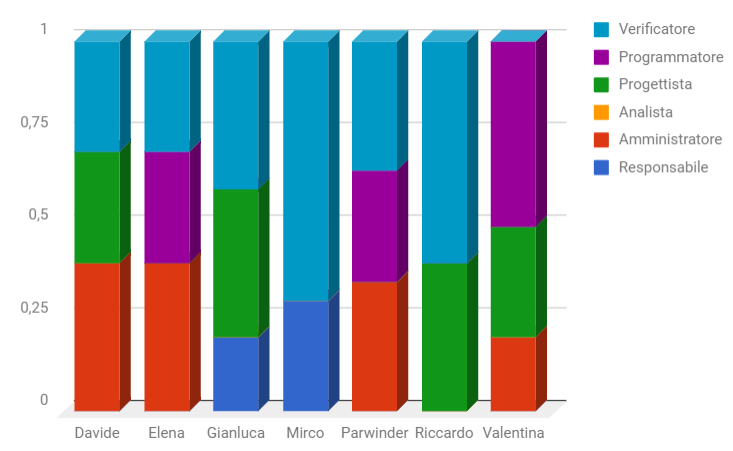
\includegraphics[width=10.5cm]{images/prospettoOrario/valCol.png}
	\label{fig:foo}
	\caption{Grafico suddivisione oraria del periodo di Validazione e collaudo}
\end{figure} 
\newpage
\subsection{Prospetto Economico}
Nel periodo di Validazione e collaudo la distribuzione delle ore tra i differenti ruoli è la seguente:
\begin{table}[H]
	\begin{center}
		\capstart
		\begin{tabu} to \textwidth { 
				>{\centering}m{0.4\linewidth} 
				>{\centering}m{.2\linewidth}  
				>{\centering\arraybackslash}m{0.25\linewidth}  }
			\tableHeaderStyle
			\textbf{Ruolo} & \textbf{Ore} & \textbf{Costo in \euro} \\
			\resp & 10 & 300,00 \\
			\amme & 27 & 540,00 \\
			\alista &  &  \\
			\proga & 28 & 616,00 \\
			\progre & 36 & 540,00 \\
			\vere & 39 & 585,00 \\
			\textbf{Totale} & \textbf{140} & \textbf{2.581,00} \\
		\end{tabu}
		\caption{Prospetto economico del periodo di Verifica e collaudo}
		\vspace{-1em}
	\end{center}
\end{table}

Il seguente grafico dà una rappresentazione visiva della distribuzione dei ruoli:
\begin{figure}[h]
	\centering
	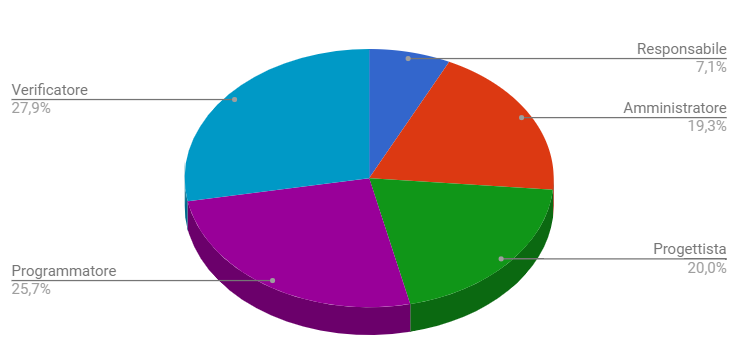
\includegraphics[width=12.5cm]{images/prospettoEconomico/valCol.png}
	\label{fig:foo}
	\caption{Grafico suddivisione dei ruoli del periodo di Validazione e collaudo}
\end{figure} 
\clearpage
\section{Totale ore rendicontate}
\subsection{Totale suddivisione ore rendicontate}
Di seguito sono riportate il totale delle sole ore rendicontate nel preventivo a carico del committente:


Il seguente grafico dà una rappresentazione visiva della suddivisione oraria:\\
\begin{figure}[h]
	\centering
	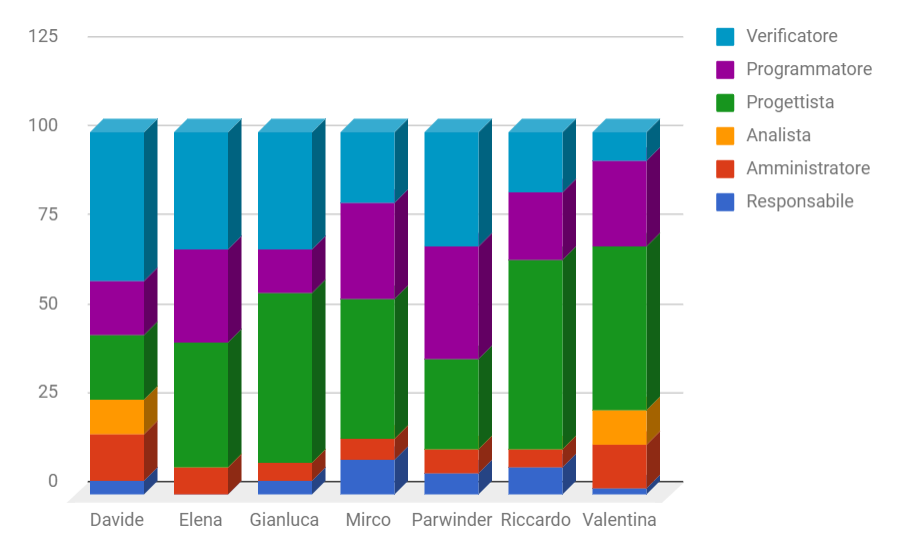
\includegraphics[width=10cm]{images/prospettoOrario/totRen.png}
	\label{fig:foo}
	\caption{Grafico suddivisione oraria totale delle ore rendicontate}
\end{figure} 
\clearpage
\subsection{Totale del prospetto economico rendicontato}
Di seguite è riportato il totale delle ore dei diversi ruoli del progetto contando solo le ore rendicontate nel preventivo a carico del committente cioè dei periodi di Progettazione architetturale, Progettazione di dettaglio e codifica e il periodo di Validazione e collaudo:


Il seguente grafico dà una rappresentazione visiva della distribuzione dei ruoli:
\begin{figure}[h]
	\centering
	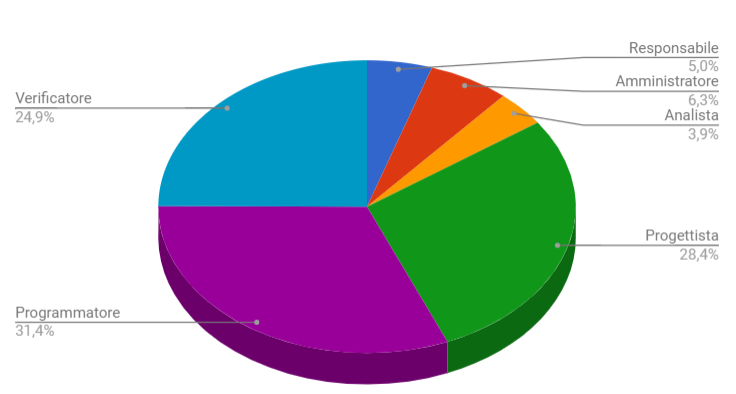
\includegraphics[width=10.5cm]{images/prospettoEconomico/totRen.png}
	\label{fig:foo}
	\caption{Grafico suddivisione dei ruoli totale delle ore rendicontate}
\end{figure} 
\clearpage
\section{Totale ore con investimento}
\subsection{Totale suddivisione ore con investimento}
Di seguito sono riportate il totale delle ore del progetto contando le ore di investimento e delle ore rendicontate nel preventivo a carico del committente:


Il seguente grafico dà una rappresentazione visiva della suddivisione oraria:
\begin{figure}[h]
	\centering
	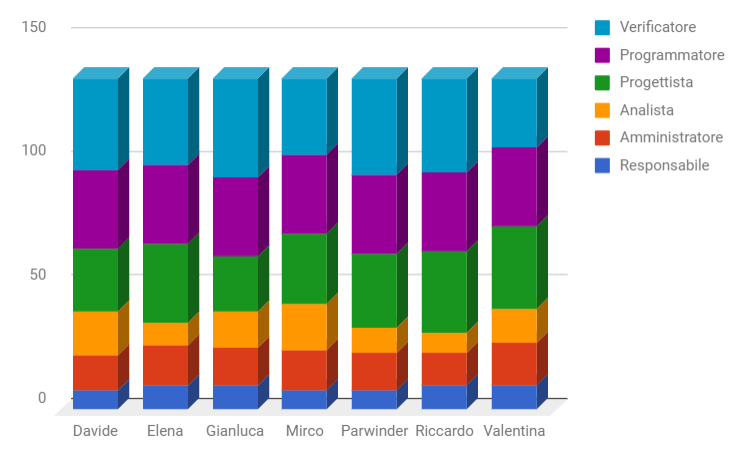
\includegraphics[width=10.5cm]{images/prospettoOrario/totale.png}
	\label{fig:foo}
	\caption{Grafico suddivisione oraria totale delle ore di investimento e rendicontate}
\end{figure} 
\clearpage
\subsection{Totale del prospetto economico con investimento}
Di seguito è riportato il totale delle ore dei diversi ruoli del progetto contando le ore di investimento e delle ore rendicontate nel preventivo a carico del committente:


Il seguente grafico dà una rappresentazione visiva della distribuzione dei ruoli:
\begin{figure}[ht]
	\centering
	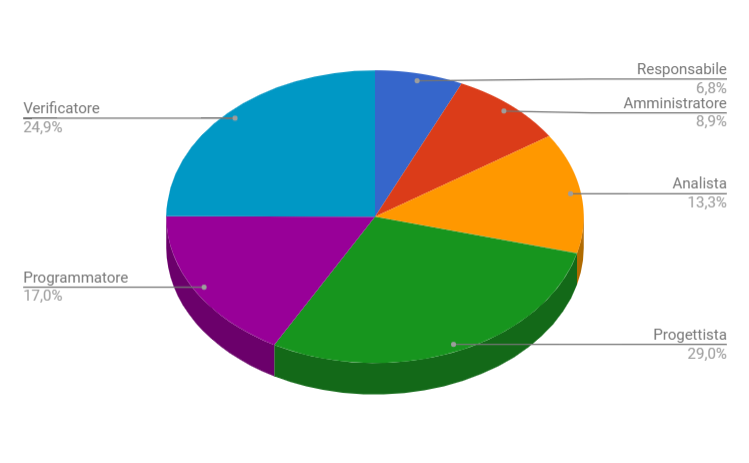
\includegraphics[width=10.5cm]{images/prospettoEconomico/totInv.png}
	\label{fig:foo}
	\caption{Grafico suddivisione totale dei ruoli delle ore di investimento e rendicontate}
\end{figure} 

\end{document}